\begin{enumerate}
\item The normal vector of the altitude from $\vec{A}$ is,
\begin{align}
\vec{m}_{BC}
= \myvec{1\\-1},
\because \vec{n}_{BC} &= \myvec{1\\1}.
\end{align}
The equation of the desired altitude  is given by
\begin{align}
\vec{m}_{BC}^{\top}\vec{x} &=\vec{m}_{BC}^{\top}\vec{A}\\
\implies \myvec{1&-1}\vec{x} &= -1
\end{align}
	\item
The equation of line $BC$ is given by,
\begin{align}
{\vec{n}^{\top}_{BC}}\vec{x} &= {\vec{n}^{\top}_{BC}}\vec{B}\\
\implies \myvec{1&1}\vec{x}  &= 3
\end{align}
			From \eqref{eq:PQ-final},
the length of the desired altitude is 
\begin{align}
d =  \sqrt{2}
\end{align}

\end{enumerate}
See 
\figref{fig:chapters/11/10/3/17/1}.
\begin{figure}[ht]
\centering
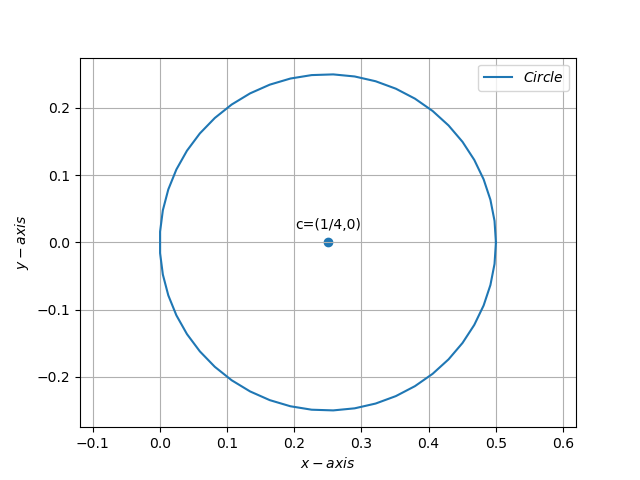
\includegraphics[width = \columnwidth]{chapters/11/10/3/17/figs/fig.png}
\caption{}
\label{fig:chapters/11/10/3/17/1}
\end{figure}
